In this chapter we come to the core of this thesis, namely the empirical performance investigation of the Fribourg construction. We are interested in two things. First, how the different versions of the Fribourg construction compare to each other. That is, how do different combinations of optimisations influence the performance of the construction. Second, we want to know how the Fribourg construction performs compared to existing complementation constructions. Our main measure for the performance of a construction is the number of states of the produced complement. Throughout this thesis, we will refer to the first question as the \textit{internal} tests, and to the second question as the \textit{external} tests.

To do an empirical performance investigation we need an implementation of the Fribourg construction. We decided to create this implementation in the framework of an existing tool called \goal. This is a Java tool with a graphical user interface for manipulating \om-automata, and it contains implementations of various Büchi complementation constructions. In this way we can easily compare the Fribourg construction to these other construction (see external tests).

The next thing we need for an empirical performance investigation is test data. These are specific sets of automata on which all the tested construction are run. We defined two test sets. The first one, called the \goal{} test set, contains a large number of randomly generated automata. The second one, called the Michel test set, contains just a small number of automata that have a special property.

Having an implementation and test data, the experiments need to be executed. Our chosen implementation approach and test data results in heavy computation tasks, that require a lot of computation power and time. We therefore decided to execute the experiments in a professional high-performance computing (HPC) environment. This environment is the Linux-based HPC computing cluster, called UBELIX, at the University of Bern.\footnote{\url{http://ubelix.unibe.ch}}

In this chapter, we describe each of these points in a separate section. Section~\ref{4_exp_setup} also includes our experimental setup, that is, a listing of the concrete construction versions that we tested, the allocated computing resources, and so on. The results of the experiments will finally be presented in Chapter~\ref{chap_results}.


\section{Implementation}
As mentioned, we implemented the Fribourg construction as part of the \goal{} tool. This is possible thanks to the extensible plugin architecture of \goal{} which allows to write plugins that contain additional functionality for \goal. Our implementation of the Fribourg construction has therefore the form of a \goal-plugin.

In this section, we first present the \goal{} tool in a general way (Section~\ref{4_goal}). In Section~\ref{4_implementation}, we give some more details about the plugin architecture of \goal, and describe some properties of our implementation. Finally, in Section~\ref{4_verification}, we describe how we verified the correctness of our implementation.


\subsection{GOAL}
\label{4_goal}
\goal{} stands for \textit{Graphical Tool for Omega-Automata and Logics} and is being developed since 2007 by the Department of Information Management at the National Taiwan University (NTU)\footnote{\url{http://exp.management.ntu.edu.tw/en/IM}}. The tool has been presented in various scientific publications~\cite{2007_goal}\cite{2008_goal_ext}\cite{2009_goal}\cite{2013_goal}. It is a Java program, and it is freely available on \url{http://goal.im.ntu.edu.tw}.

\goal{} is an \om-automata manipulation tool. It provides a large number of operations that can be applied to different types of \om-automata. These operations range from input testing, conversions to other types of automata, to union and intersection. Figure~\ref{goal_gui} shows a screenshot of \goal's graphical user interface with an open menu showing the breadth of operations that \goal{} provides. Of course, complementation is also part of these operations, and \goal{} includes a some of well-known Büchi complementation constructions, that we will describe below.

\begin{figure}[htb!]
\centering
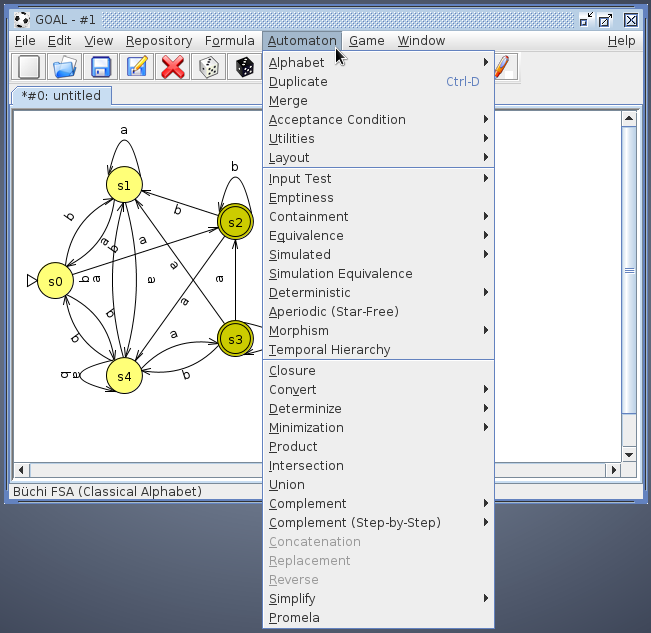
\includegraphics[width=0.45\textwidth]{figures/goal.png}
\caption{The graphical user interface of \goal{} (version 2014--11--17). The open menu item gives an idea about the different types of manipulations that \goal{} provides for \om-automata.}
\label{goal_gui}
\end{figure}

Automata can be imported to and exported from \goal{} in different formats. The default format is the \goal{} File Format (GFF), and files of this type have conventionally the extension ``.gff''. 

The main interface of \goal{} is a graphical one, as shown in Figure~\ref{goal_gui}. However, almost the entire functionality of \goal{} is also available through a command line interface. Complementing an automaton can then for example be done with the command \textsf{gc complement -m safra -o out.gff in.gff}. This would complement the automaton in the file \textsf{in.gff} with the Safra construction, and write the complement in the \goal{} File Format to the file \textsf{out.gff}. The command \textsf{gc} is the \goal{} executable for the command line interface. The command line interface is a very important feature that makes \goal{} usable for automated batch processing.

\goal{} is versioned by version names of the form YYYY--MM--DD that specify the release date. The latest version at the time of this writing is version 2014--11--17. This is the version that our description is based on, and that we used for all our experiments.

What we are most interested in, in the context of this thesis, are of course \goal's Büchi complementation constructions. The the 2014--11--17 version of \goal{}, contains implementations of 10 Büchi complementation constructions that are well-known from the literature. Table~\ref{goal_constructions} lists these constructions together with their authors and reference to the literature.

\begin{table}[htb!]
\centering
\begin{tabular}{rlllr}
\hline
\# & Identifier & Name/description & Authors (year) & Ref. \\
\hline
1 & Ramsey & Ramsey-based construction & Sistla, Vardi, Wolper (1987) & \cite{PrasadSistla1987217} \\
2 & Safra & Safra construction & Safra (1988) & \cite{1988_safra_1} \\
3 & ModifiedSafra & Modification by Althoff & Althoff (2006) & \cite{2006_althoff} \\
4 & Piterman & Safra-Piterman construction & Piterman (2007) & \cite{2007_piterman} \\
5 & MS & Muller-Schupp construction & Muller, Schupp (1995) & \cite{Muller199569} \\
6 & Rank & Rank-based construction & Schewe (2009) & \cite{schewe2009buchi} \\
7 & WAPA & Via weak alternating parity automata & Thomas (1999) & \cite{1999_thomas} \\
8 & WAA & Via weak alternating automata & Kupferman, Vardi (2001) & \cite{Kupferman:2001} \\
9 & Slice+P & Slice-based construction (earlier) & Vardi, Wilke (2007) & \cite{vardi2007automata} \\
10 & Slice & Slice-based construction (later) & Kähler, Wilke (2008) & \cite{2008_kaehler} \\
\hline
\end{tabular}
\caption{The pre-implemented NBW complementation constructions in \goal{} (version 2014-11-17).}
\label{goal_constructions}
\end{table}

We sorted the construction in Table~\ref{goal_constructions} according to the four fundamental complementation approaches, Ramsey-based, determinization-based, rank-based, and slice-based. The first construction, Ramsey, is the only construction belonging to the Ramsey-based complementation approach. The following four constructions, Safra, ModifiedSafra, Piterman, and MS, belong to the determinization-based approach. Rank, WAPA, and WAA belong to the rank-based approach. Finally, Slice and Slice+P belong to the slice-based approach. Throughout the rest of this thesis, when we refer to one of \goal's Büchi complementation constructions, we will use the identifiers as defined in Table~\ref{goal_constructions}.

Slice and Slice+P are actually combined in a single construction in \goal. However, one of the two constructions can be selected by the means of the option P. With the P option, the construction by Vardi and Wilke is used, and without the P option, the one by Kähler and Wilke is used. For our study, we will use Vardi and Wilke's construction (with the P option), however, we will usually still refer to this construction as simply Slice.

At this point, it is worth pointing at a related project of the same research group, called the Büchi Store. This is an online repository of classified and tagged \om-automata that can be downloaded in different formats (including GFF). The Büchi Store is located on \url{http://buchi.im.ntu.edu.tw/} and has also been described in a scientific publication~\cite{2011_buchi_store}. Furthermore, there is a binding in \goal{} to the Büchi Store, so that the contents of the store can be directly accessed from \goal{}. For our project we did not make use the Büchi Store, but it is might be an interesting option for related projects.


\subsection{Implementation of the Construction}
\label{4_implementation}
\subsubsection{The \goal{} Plugin}
\goal{} has been designed from the ground up to be modular and extensible. To this end, it has been created with the Java Plugin Framework (JPF)\footnote{\url{http://jpf.sourceforge.net/}}. This framework allows to build applications whose functionality can be easily and seamlessly extended by writing additional plugins for it. These plugins can be installed in the main application without the need to recompile the whole application. Rather, the plugin is compiled separately and the resulting bytecode files are copied to the directory tree of the main application. It is not even necessary to know the source code of the main application in order to write a plugin. The interfaces of JPF itself, and the documentations of the relevant classes of the main application are all that a plugin writer needs to know.

In some more detail, JPF requires an application to define so called \textit{extension points}. For any extension point, multiple \textit{extensions} can be provided. These extensions contain the actual functionality of the application. A JPF application basically consists of extensions that are plugged into their corresponding extension points. A plugin is an arbitrary bundle of extensions and extension points. It is the basic unit of organisation in the Java Plugin Framework.

One of the extension points of \goal{} is called \textsf{ComplementConstruction}. The extensions to \textsf{ComplementConstruction} contain the actual complementation constructions that \goal{} provides. For adding a new complementation construction to \goal, one has thus to create a new extension to \textsf{ComplementConstruction}. This extension can then be wrapped in a plugin, and the plugin can be compiled and installed in the main application, what makes it an integral part of it. This means that once the plugin is installed, the new construction is included in \goal{} in the same way as all the other constructions.

This is how we added the Fribourg construction to \goal. The name of our plugin is \textsf{ch.unifr.goal.complement}\footnote{By convention, JPF plugins are named after the base package name of their implementation files.}. It is publicly available and can be installed by anybody in their \goal{} application. We give instructions on how to get, install, and use the plugin in Appendix~\ref{app_plugin}.

In reality, there is more than just the extension point \textsf{ComplementConstruction} that can be extended to add a new complementation construction to \goal. There are separate extension points for, for example, the command line binding, menu inclusion, or step-by-step execution support. We created extensions to all these extension points as well and included them in our plugin. Our aim was to make the integration of the Fribourg construction in \goal{} as complete as possible so that it provides the same facilities as the pre-implemented constructions.

\subsubsection{The Fribourg Construction Options}
In our implementation of the Fribourg construction we also included the three optimisations, R2C, M1, and M2, described in Section~\ref{3_optimisations}. We implemented these optimisation as user-selectable complementation construction options. In the GUI, these options are presented to the user as a list of checkboxes immediately before the start of each complementation task. In the command line mode, there is a command line flag for each option that can be set or not set by the user.

In addition to the three optimisations, we added further options to our construction. Table~\ref{goal_options} lists all the available options for the Fribourg construction. Each option has an identifier consisting of upper-case letters that we will use throughout the rest of this thesis to refer to the corresponding options.

\begin{table}
\centering
\begin{tabular}{ll}
\hline
Option & Description \\
\hline
R2C & Apply R2C optimisation if input automaton is complete \\
M1 & Apply M1 optimisation (component merging) \\
M2 & Apply M2 optimisation (colour 2 reduction) \\
C & Make input automaton complete before start of construction \\
R & Remove unreachable and dead states from output automaton \\
RR & Remove unreachable and dead states from input automaton \\
MACC & Maximise accepting states of input automaton \\
B & Use the ``bracket notation'' for state labels \\
\hline
\end{tabular}
\caption{The options of the Fribourg construction in \goal.}
\label{goal_options}
\end{table}

The first three options in Table~\ref{goal_options} represent the three optimisations from Section~\ref{3_optimisations}. The R2C optimisation is implemented so that it applies only to input automata that are complete. That is, selecting R2C for the complementation of an automaton that is not complete has no effect, and the result is the same as if R2C would not have been selected. The options M1 and M2 implement the M1 and M2 optimisations. Since M2 is dependent on M1, it is not possible to select M2 without also selecting M1. This restriction is enforced in both the GUI and the command line interface.

The C option is one of the options that modifies the input automaton before the actual complementation starts. This option first checks if the input automaton is complete\footnote{An automaton is complete if every state has at least one outgoing transition for every symbol of the alphabet.}, and if this is not the case, makes it complete by adding a sink state. This means that an additional non-accepting state, the sink state, is added to the automaton, and from every incomplete state the ``missing'' transitions are added from this state to the sink state. The sink state itself has loop transitions for all symbols of the alphabet.

The purpose of the C option is to be used in conjunction with the R2C optimisation. By making an automaton complete before the start of the construction, we can ensure that the R2C optimisation will be applied. The question then arises whether, in terms of performance, it is worth to do is. Because for making an automaton complete, we have to add an additional state to the automaton what generally increases the complexity of the complementation. This question has been investigated in previous work about the Fribourg construction by Göttel~\cite{2013_bsc_goettel}. In this thesis will re-investigate this point in an extended form.

The R option modifies the output automaton at the end of the construction. In particular, it removes all the so called unreachable and dead states from the complement. Unreachable states are states that cannot be reached from the initial state. Dead states are states from which it is not possible to reach an accepting state. These states can be removed from any automaton without changing the language of the automaton. The pre-implemented complementation constructions Ramsey, Piterman, Rank, and Slice also contain a similar R option.

One usage case of the R option is to determine the number of unreachable and dead state that a complementation construction produces. Complementing the same automaton with and without the R option, and taking the difference of the complement sizes will yield this number. Investigations in this direction have been done with \goal{} by Tsai~et~al.~\cite{2011_tsai}. In our own investigations we will use the R option to determine the number of unreachable and dead states the plain Fribourg construction produces.

The RR option is similar to the R option, except that it removes the unreachable and dead states from the input automaton rather than from the output automaton. This option is a custom creation by us, and the pre-implemented complementation constructions in \goal{} do not contain a similar option. We are not using the RR option in our investigations.

The MACC option again modifies the input automaton before the start of the construction. Namely, it applies the technique of the ``maximisation of the accepting set''. This means that as many states as possible are made accepting without changing the language of the automaton. The larger number of accepting state should then simplify the complementation task. This technique has been introduced and empirically investigated by Tsai~et~al. in~~\cite{2011_tsai}. The pre-implemented complementation constructions Ramsey, Piterman, Rank, and Slice contain a similar MACC option. In our own investigations we will however not use the MACC option.

Finally, the B option is a pure display option and does not alter the automata or the construction itself. Its effect is to use the bracket notation for state labels, that indicates component colours by different types of brackets, instead of the default notation that uses numbers to specify the component colours.


\subsection{Verification of the Implementation}
\label{4_verification}
% Results on  UBELIX/jobs/2014-11-25
Having an implementation, it is important to verify that it is correct. With correct we mean in this section that the construction produces a valid complement for a given input automaton, that is, that the language of the output automaton is indeed the complement of the language of the input automaton. We verified this point of our implementation as described below. In this sense, we know that our implementation is a valid construction. This is not the same as the verification that our implementation faithfully represents the Fribourg construction as it has been devised by its creators. Rather, this latter point has been informally verified during the whole development period of the implementation, which was possible thanks to the close collaboration with the construction creators.

In order to verify that our implementation produces correct results, we performed so called complementation-equivalence tests in \goal{} against one of the pre-implemented construction. This works as follows. Take an automaton $A$ and complement it with one of the \goal{} constructions. This yields automaton $A^\prime$. Then, complement the same automaton $A$ with our implementation of the Fribourg construction. This yields automaton $A^{\prime\prime}$. Now, by the means of \goal's equivalence operation then test whether $A^\prime$ and $A^{\prime\prime}$ accept the same language.

This approach makes a couple of assumptions. First, it relies on the correctness of the pre-implemented complementation constructions, and on the equivalence operation of \goal{} (which is also based on complementation). Second, with this empirical approach it is of course not possible to conclusively verify the correctness of our implementation. Every passed complementation-equivalence test just further confirms the hypothesis that our implementation is correct, but it can never be proved. Despite these points, we think that this approach is the best we can do, and that, with a sufficient number of test cases, it can confirm the correctness of our implementation with a high probability.

We tested the Fribourg construction in different versions with all the options that we described in the last section (except the B option as it does not influence the construction). The tested versions are the following.
\begin{itemize}
\item Fribourg
\item Fribourg+R2C+C
\item Fribourg+M1
\item Fribourg+M1+M2
\item Fribourg+R
\item Fribourg+RR
\item Fribourg+MACC
\end{itemize}

We tested each version with 1,000 randomly generated automata. The automata had a size of 4 and an alphabet size between 2 and 4. The pre-implemented construction we tested against, was the Piterman construction. The computations were executed on the UBELIX computer cluster that is described in Section~\ref{4_exec_env}. The result was that all the tests were successful, that is, there was not a single counterexample.

With a size of 4, the automata used for the tests are rather small, and it would be interesting to do the tests with bigger automata. However, our limited computing and time resources prevented us from doing so. The equivalence test of \goal{} is implemented as reciprocal containment tests, which include complementation. That is, the overall test includes the complementation of the complements of the test automata. By using bigger test automata, their complements might be already so big that a further complementation is practically infeasible with our available resources. Nevertheless, we think that the high number of performed tests confirms the correctness of our construction with a high probability.


\section{Test Data}
Test data is the sample data that is given to an algorithm as input in order to measure and evaluate certain properties of the output. The test data is an important part of every empirical study and should meet several requirements. It should include enough test cases so that the results are statistically significant. It should not be biased in favour of the tested algorithm. It should cover test scenarios that are relevant for evaluating the performance of the algorithm. Ideally, publicly available test data is used that has also  been used for other empirical studies. In this way, the data is ``objective'' and results of different studies are comparable.

In our case the test data consists of a set of non-deterministic Büchi automata which are provided as input to the Fribourg construction. We chose two different sets of automata of which we believe that together they form a meaningful test set for our study.

The first set of test automata, which we call \goal{} test set, consists of 11,000 NBW of size 15. This test set has been used by a previous empirical study with \goal{} by Tsai~et~al.~\cite{2011_tsai}, and is publicly available. The second set of automata, which we call Michel test set, consists of a family of automata that show a very pronounced state growth for complementation. These automata have been introduced and described by Michel~\cite{michel1988}, hence the name. Below, we describe these two test sets with their relevant properties in separate sections.


\subsection{GOAL Test Set}
\label{4_goal_testset}
The \goal{} test set is the larger and more complex one of the two test sets. In this section, we first introduce the \goal{} test set and describe its basic structure. In the second part, we present the results of an analysis that we did in order to reveal further properties of the \goal{} test set, namely the number and distribution of complete, universal, and empty automata.

\subsubsection{Introduction and Basic Structure}
The \goal{} test set has been created by Tsai~et~al. for an empirical study evaluation the effects of several optimisations on existing Büchi complementation constructions~\cite{2011_tsai}. This study has been executed in \goal{} and the automata in the test set are available in the \goal{} file format, hence the name \goal{} test set.

The entire test set consists of 11,000 automata of size 15, and 11,000 similar automata of size 20. For our study we used however only the automata of size 15. Hence, when we refer to the \goal{} test set in the rest of this thesis, we specifically mean the 11,000 automata of size 15. The \goal{} test set is publicly available through the following link: \url{https://fribourg.s3.amazonaws.com/testset/goal.zip}\footnote{This link is maintained by the author of the thesis. The original link of the \goal{} tests set that is maintained by the authors of~\cite{2011_tsai} is \url{http://goal.im.ntu.edu.tw/wiki/lib/exe/fetch.php?media=goal:ciaa2010_automata.tar.gz}. This package contains additionally the 11,000 automata of size 20. In the package of the first link, the files have been renamed, however, the content of the files has not been changed.}.

All the automata in the test set have 15 states and an alphabet size of 2. The further properties of the automata, namely accepting states and transitions, are determined by the values of two parameters called \textit{transition density} and \textit{acceptance density}

The transition density determines the number of transitions of an automaton. In some more detail, the transition density $t$ is defined as follows. Let $n$ be the number of states of automaton $A$, and $t$ its transition density. Then $A$ contains $tn$ transitions for each symbol of the alphabet. In the case that $tn$ is not an integer, it is rounded up to the next integer. That is, if one of our automata with 15 states and the alphabet ${0, 1}$ has a transition density of 2, then it contains exactly 30 transitions for symbol $0$ and 30 transitions for symbol $1$. %At creation time the start and end points of these transitions are chosen at random. %Consequently, each state has on average two outgoing and two incoming transitions for each symbol. Therefore, the transition density can also be seen as the average number of outgoing and incoming transitions per alphabet symbol that a state has.

The acceptance density $a$ is defined as the ratio of accepting states to non-accepting states in the automaton. It is thus a number between 0 and 1. If automaton $A$ has $n$ states and an acceptance density of $a$, then it has $an$ accepting states. In the case that $an$ is not an integer, it is rounded up to the next integer. %Which $an$ states are made accepting is determined randomly at creation time.

The \goal{} test set is structured into 110 classes with different transition density/acceptance density pairs. These 110 pairs result from the Cartesian product of 11 transition densities and 10 acceptance densities. The concrete transition densities $t^\prime$ and acceptance densities $a^\prime$ are the following:
\begin{align*}
t^\prime & = \left( 1.0,\,1.2,\,1.4,\,1.6,\,1.8,\,2.0,\,2.2,\,2.4,\,2.6,\,2.8,\,3.0 \right) \\
a^\prime & = \left( 0.1,\,0.2,\,0.3,\,0.4,\,0.5,\,0.6,\,0.7,\,0.8,\,0.9,\,1.0 \right)
\end{align*}
Thus, there is one class whose automata have a transition density of 1.0 and an acceptance density of 0.1, another class with a transition density of 1.0 and an acceptance density of 0.2, and so on. Each of the 110 classes contains 100 automata

When Tsai~et~al. created the \goal{} test set, they created the automata within the given constraints of any class at random. They chose this structure and parameter values in order to generate a broad range of complementation problems ranging from easy to hard~\cite{2011_tsai}.


\subsubsection{Further Properties: Completeness, Universality, and Emptiness}

\renewcommand{\tabcolsep}{0.05cm}   % Change table spacings
\renewcommand{\arraystretch}{1.05}
\newcolumntype{R}{>{\raggedleft\arraybackslash}p{1.5em}}
\begin{figure}[htb!]
  \centering
  \begin{subfigure}{\textwidth}
    \begin{subtable}{0.47\textwidth}
    % latex table generated in R 3.1.2 by xtable 1.7-4 package
% Sun Aug 16 12:48:04 2015
\begin{tabular}{r|RRRRRRRRRR}
  & 0.1 & 0.2 & 0.3 & 0.4 & 0.5 & 0.6 & 0.7 & 0.8 & 0.9 & 1.0 \\ 
  \hline
1.0 & 0 & 0 & 0 & 0 & 0 & 0 & 0 & 0 & 0 & 0 \\ 
  1.2 & 0 & 0 & 0 & 0 & 0 & 0 & 0 & 0 & 0 & 0 \\ 
  1.4 & 0 & 0 & 0 & 0 & 0 & 0 & 0 & 0 & 0 & 0 \\ 
  1.6 & 0 & 0 & 0 & 0 & 0 & 0 & 0 & 0 & 0 & 0 \\ 
  1.8 & 1 & 1 & 0 & 0 & 0 & 1 & 1 & 1 & 0 & 0 \\ 
  2.0 & 0 & 5 & 1 & 2 & 2 & 3 & 1 & 2 & 2 & 2 \\ 
  2.2 & 5 & 10 & 8 & 5 & 3 & 5 & 8 & 6 & 7 & 1 \\ 
  2.4 & 10 & 6 & 11 & 11 & 8 & 6 & 10 & 20 & 9 & 7 \\ 
  2.6 & 17 & 17 & 12 & 16 & 14 & 19 & 22 & 21 & 19 & 19 \\ 
  2.8 & 27 & 20 & 29 & 32 & 26 & 27 & 30 & 25 & 24 & 19 \\ 
  3.0 & 37 & 37 & 40 & 39 & 34 & 37 & 38 & 35 & 38 & 39 \\ 
  \end{tabular}

    \end{subtable}
    \hfill
    \begin{subfigure}{0.52\textwidth}
    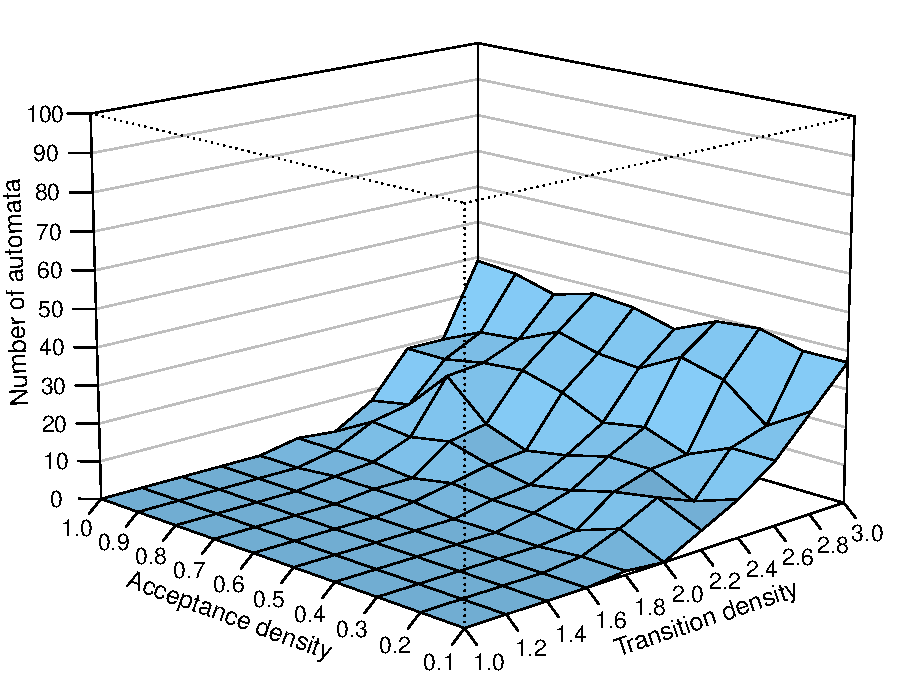
\includegraphics[width=\textwidth]{figures/r/testset/compl.persp.pdf}
    \end{subfigure}
  \caption{Number of \textit{complete} automata per class.}
  \end{subfigure}

 \begin{subfigure}{\textwidth}
    \begin{subtable}{0.47\textwidth}
    % latex table generated in R 3.1.2 by xtable 1.7-4 package
% Sun Aug 16 12:48:04 2015
\begin{tabular}{r|RRRRRRRRRR}
  & 0.1 & 0.2 & 0.3 & 0.4 & 0.5 & 0.6 & 0.7 & 0.8 & 0.9 & 1.0 \\ 
  \hline
1.0 & 4 & 5 & 5 & 7 & 8 & 4 & 6 & 10 & 4 & 3 \\ 
  1.2 & 1 & 3 & 5 & 8 & 8 & 12 & 10 & 13 & 4 & 14 \\ 
  1.4 & 2 & 17 & 13 & 17 & 20 & 24 & 22 & 21 & 27 & 26 \\ 
  1.6 & 16 & 28 & 30 & 37 & 49 & 42 & 42 & 49 & 45 & 45 \\ 
  1.8 & 31 & 40 & 55 & 59 & 64 & 67 & 76 & 70 & 63 & 78 \\ 
  2.0 & 60 & 64 & 85 & 75 & 83 & 83 & 79 & 90 & 87 & 83 \\ 
  2.2 & 67 & 87 & 86 & 88 & 89 & 91 & 89 & 89 & 89 & 86 \\ 
  2.4 & 88 & 89 & 86 & 92 & 95 & 95 & 94 & 97 & 96 & 97 \\ 
  2.6 & 86 & 93 & 92 & 97 & 97 & 97 & 98 & 96 & 98 & 96 \\ 
  2.8 & 94 & 97 & 95 & 94 & 97 & 99 & 98 & 97 & 97 & 100 \\ 
  3.0 & 99 & 99 & 99 & 97 & 99 & 98 & 100 & 100 & 100 & 99 \\ 
  \end{tabular}

    \end{subtable}
    \hfill
    \begin{subfigure}{0.52\textwidth}
    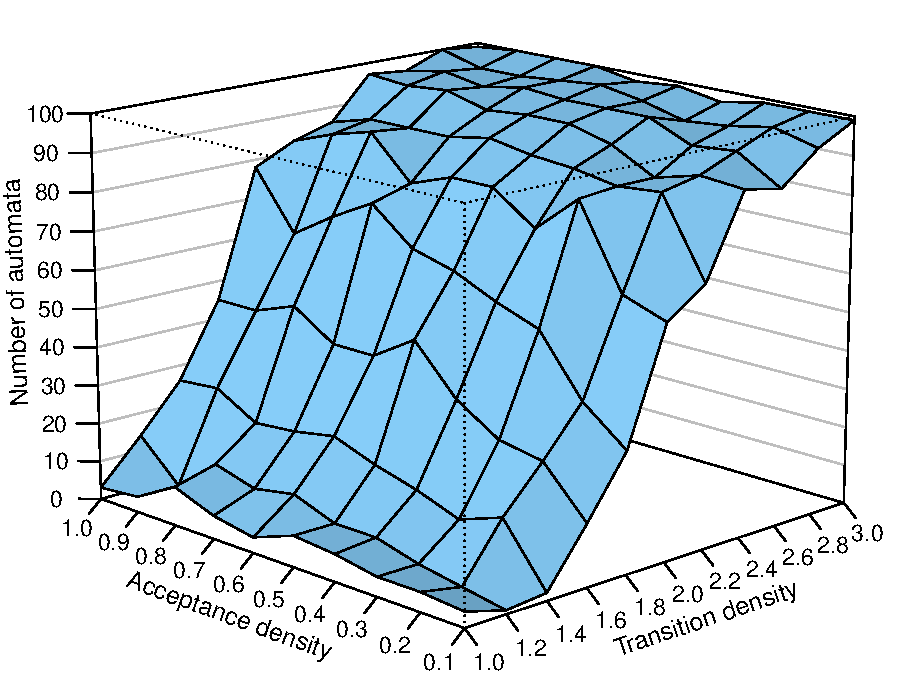
\includegraphics[width=\textwidth]{figures/r/testset/univ.persp.pdf}
    \end{subfigure}
  \caption{Number of \textit{universal} automata per class}
  \end{subfigure}

  \begin{subfigure}{\textwidth}
    \begin{subtable}{0.47\textwidth}
    % latex table generated in R 3.1.2 by xtable 1.7-4 package
% Sun Aug 16 12:48:05 2015
\begin{tabular}{r|RRRRRRRRRR}
  & 0.1 & 0.2 & 0.3 & 0.4 & 0.5 & 0.6 & 0.7 & 0.8 & 0.9 & 1.0 \\ 
  \hline
1.0 & 17 & 7 & 4 & 5 & 2 & 4 & 3 & 1 & 1 & 0 \\ 
  1.2 & 4 & 2 & 1 & 1 & 0 & 1 & 0 & 0 & 0 & 0 \\ 
  1.4 & 2 & 1 & 0 & 0 & 0 & 0 & 0 & 0 & 1 & 2 \\ 
  1.6 & 0 & 0 & 0 & 0 & 0 & 0 & 1 & 0 & 0 & 0 \\ 
  1.8 & 1 & 0 & 0 & 0 & 1 & 0 & 0 & 0 & 0 & 0 \\ 
  2.0 & 0 & 0 & 0 & 0 & 0 & 0 & 0 & 0 & 0 & 0 \\ 
  2.2 & 0 & 0 & 0 & 0 & 0 & 0 & 0 & 0 & 0 & 0 \\ 
  2.4 & 0 & 0 & 0 & 0 & 0 & 0 & 0 & 0 & 0 & 0 \\ 
  2.6 & 0 & 0 & 0 & 0 & 0 & 0 & 0 & 0 & 0 & 0 \\ 
  2.8 & 0 & 0 & 0 & 0 & 0 & 0 & 0 & 0 & 0 & 0 \\ 
  3.0 & 0 & 0 & 0 & 0 & 0 & 0 & 0 & 0 & 0 & 0 \\ 
  \end{tabular}

    \end{subtable}
    \hfill
    \begin{subfigure}{0.52\textwidth}
    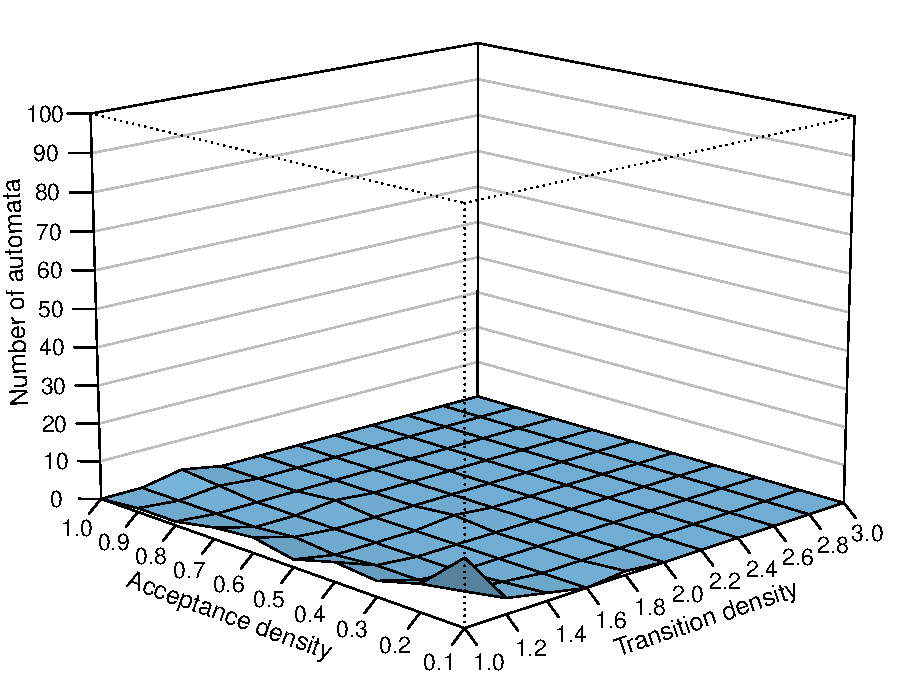
\includegraphics[width=\textwidth]{figures/r/testset/empt.persp.pdf}
    \end{subfigure}
  \caption{Number of \textit{empty} automata per class}
  \end{subfigure}
\caption{Number of complete, universal, and empty automata for each of the 110 classes of transition density/acceptance density combinations. Each class contains 100 automata.}
\label{testset_analysis}
\end{figure}
\tablestyle  % Reset old table spacings

We analysed the properties of completeness, universality, and emptiness\footnote{An automaton is \textit{complete} if every state has at least one outgoing transition for every symbol of the alphabet. An automaton is \textit{universal} if it accepts every word that can be generated from its alphabet. An automaton is \textit{empty} if it does not accept anything (except the empty word $\epsilon$).} of the automata in the \goal{} test set. To know about these properties is useful for the interpretation of the results of our study. For example, the R2C optimisation applies only to complete automata, thus it is interesting to know how many automata are complete. The smallest possible complements of universal and empty automata have a size of 1. Thus, we can see how many ``superfluous'' states a construction produces when complementing a universal or empty automaton.

\goal{} provides a command for testing emptiness. However, it does not provide commands for testing completeness and universality. We therefore implemented these commands on our own and bundled them as a separate \goal{} plugin. The plugin is called \textsf{ch.unifr.goal.util} and also publicly available as described in Appendix~\ref{app_plugin}.

With these \goal{} commands we tested each of the 11,000 automata for the three properties. On one hand, we want to know how many complete, universal, and empty automata are there in total. On the other hand, we also want to know how these properties are distributed across the 110 classes of transition density/acceptance density combinations. Thus, we also determined the number of complete, universal, and empty automata for each class. The computations were executed on the UBELIX computer cluster that is described in Section~\ref{4_exec_env}.

The resulting overall numbers are the following:
\begin{itemize}
\item 990 of the 11,000 automata are complete (9\%)
\item 6,796 of the 11,000 automata are universal (61.8\%)
\item 63 of the 11,000 automata are empty (0.6\%)
\end{itemize}

The fact that only 9\% of the automata are complete means that the R2C optimisation of the Fribourg construction affects only 9\% of the test data. This is an interesting fact for the analysis of the effect the R2C optimisation has on the overall performance of the construction. A surprisingly high number of 61.8\% of the automata are universal. A reason might be the small alphabet of the \goal{} test set automata, which has just two symbols. With a certain number of transitions in the automata, there seems to be a high probability that the automata are universal. Conversely, the number of empty automata is very low. This can be seen as the reverse of the same effect that causes the number of universal automata to be high.

In Figure~\ref{testset_analysis}, we show the number of complete, universal, an d empty automata per class. In this figure we introduce by the way two ways for representing per-class data that we will use throughout this thesis. On the left side of Figure~\ref{testset_analysis} the per-class data is represented as matrices. These matrices always have 11 rows and 10 columns, and the rows always represent the transition densities and the columns represent the acceptance densities. On the right side of Figure~\ref{testset_analysis}, the same data is visualised as so called perspective plots. The corner of the perspective plots that is closest to the viewer corresponds to the upper-left corner of the corresponding matrices. Thus, looking at a perspective plots is like looking at the corresponding matrix from the upper-left corner. The advantage of matrices is that they show all the data values explicitly. The advantage of perspective plots is that they show the patterns in the data more intuitively. When we present the results of our study in Chapter~\ref{chap_results}, we will mainly use perspective plots, however, we will give all the corresponding matrices in Appendix~\ref{app_matrices}.

Regarding the complete automata per class in Figure~\ref{testset_analysis}~(a), we can see their number increases with the transition density. Up to a transition density of 1.6 there are no complete automata at all, and then it starts to increase up to a number between 34 and 40 for the transition density of 3.0. Since each class contains exactly 100 automata, these numbers are percentages at the same time. That the number of complete automata increases with the transition density is because a higher number of transitions per alphabet symbol in the automaton increases the probability that each state has at least one outgoing transition for each alphabet symbol. For example, with a transition density of 1.0 and 15 states, the automaton contains exactly 15 transitions for each alphabet symbol. It is still possible that this automaton is complete, but the probability is very low, because there must be a one-to-one mapping of transitions and states. On the other hand, with a transition density of 3.0, there would be 45 transitions per alphabet symbol, and the probability that each state gets one of them is much higher.

The number of universal automata per class in Figure~~\ref{testset_analysis}~(b) also increases with the transition density, although much stronger. While in the classes with a transition density of 1.0, there are between 3 and 10 universal automata, in the classes with a transition density of 3.0 there are between 97 and 100. As already mentioned, the small alphabet size of the \goal{} test set automata and a sufficiently high number of transitions results in a high probability that an automaton accepts every possible word, and thus is universal. In Figure~\ref{testset_analysis}~(b) we can also see that low acceptance densities result by trend in slightly fewer universal automata. This is because with fewer accepting states there is less chance that a given word is accepted. As we identified the small alphabet size as a possible reason for the high number of universal automata, it would be interesting to test how many universal automata there are in similar automata with a bigger alphabet size.

Conversely to the high number of universal automata, the number of empty automata is very low. The totally 63 empty automata are mainly concentrated in the upper-left corner of the matrix in Figure~\ref{testset_analysis}~(c). That is, the automata with a low transition density and a low acceptance density have the highest probability to no accept any word, and thus being empty. The reasons for this are basically the opposite reasons for the distribution of the universal automata.


\subsection{Michel Test Set}
\label{4_michel_testset}
The Michel test set is very different from the \goal{} test set. It consists of a family of automata, the Michel automata, which exhibit an especially heavy state growth for complementation.

Michel automata have been introduced in 1988 by Max Michel in order to prove a lower bound for the state growth of Büchi complementation of $(n-2)!$, where $n$ is the number of states of the input automaton~\cite{michel1988}\cite{1996_thomas}. Michel constructed a family of automata, characterised by the parameter $m$, that have $m+1$ alphabet symbols, and $m+2$ states. He proved that the complements of these automata cannot have less than $m!$ states. Since the number of states of the input automata is $n = m + 2$, the state growth in terms of input and output states is $(n-2)!$, which is around $(0.36n)^n$.

The state growth of Michel automata is so heavy that for practical reasons we are restricted to include only the first four Michel automata, that is the ones with $m=\{1,\dots,4\}$, in our test set. For the Michel automata with $m \geq 5$, the required time and computing power for complementing them with our implementation would by far exceed our available resources. We present some extrapolations in this direction in Section~\ref{5_internal_michel}. Despite the small number of automata in the test set, we can still obtain very interesting results from them, as we will see in Chapter~\ref{chap_results}.

The four Michel automata in our test set are shown in Figure~\ref{michel_automata}. We will call them Michel~1, Michel~2, Michel~3, and Michel~4, respectively. As mentioned, Michel automata have $m+2$ states and an alphabet size of $m+1$. Furthermore, they all have a single accepting state. Our Michel automata 1 to~4 have thus 3, 4, 5, and 6 states, and alphabet sizes of 2, 3, 4, and 5, respectively.

\newcommand{\subwidth}{0.42}
\begin{figure}[htb!]
\centering
  \begin{subfigure}[t]{\subwidth\textwidth}
  \MichelOne
  \caption{Michel 1 ($m=1$)}
  \end{subfigure}
  \begin{subfigure}[t]{\subwidth\textwidth}
  \MichelTwo
  \caption{Michel 2 ($m=2$)}
  \end{subfigure}

  \begin{subfigure}[b]{\subwidth\textwidth}
  \MichelThree
  \caption{Michel 3 ($m=3$)}
  \end{subfigure}
  \begin{subfigure}[b]{\subwidth\textwidth}
  \MichelFour
  \caption{Michel 4 ($m=4$)}
  \end{subfigure}
\caption{The Michel automata with $m = \{1,\dots,4\}$, an alphabet size of $m+1$, and $m+2$ states.}
\label{michel_automata}
\end{figure}

The interesting thing about the high complementation state-complexity of Michel automata is that they allow to ``elicit'' large number of states from the complementation constructions that we investigate in our study. In the theoretical approach to Büchi complementation, the main performance metric is the worst-case state complexity. This is the maximum number of states that a construction can produce, in function of the number of states of the input automaton. If for example a construction has a worst-case complexity of $(0.76n)^n$, then, if the input automaton has size $n$, the maximum size of the complement is $(0.76n)^n$.

Thus, if with the complementation of a Michel automata we measure a certain state growth for one of the constructions, say $(0.99n)^n$, then we can deduce that the worst-case complexity of this construction must be greater than or equal to $(0.99n)^n$. In this way, we can get an idea about the lower bounds for the worst-case complexities of our investigated constructions.

This concludes the presentation of the test data for our study. In the next section we are describe the experimental setup in which this test data is used.


\section{Experimental Setup}
\label{4_exp_setup}
In this section we describe the concrete experiments that we executed, including the allocated resources and imposed constraints. As mentioned, the experiments are divided into the internal tests and external tests. In the internal tests we compare different versions of the Fribourg construction with each other. In the external tests, we compare one (the most performant) version of the Fribourg construction with other well-known complementation constructions.

The internal and external test, are done with both, the \goal{} and the Michel test set. Thus, there are four groups of experiments: internal--\goal, internal--Michel, external--\goal, and external--Michel.

In Section~\ref{4_internal}, we present the versions of the Fribourg construction used for the internal tests. These versions differ for the \goal and the Michel test set, and we present them separately. In Section~\ref{4_external}, we present the version of the Fribourg construction used for the external tests (which is also different for the \goal and the Michel test set), and the concrete versions of the third-party construction against which we compare the Fribourg construction. In Section~\ref{4_exec_env}, we describe the computing environment in which the experiments were executed. Finally, in Section~\ref{4_limits}, we present the time and memory limits that were imposed on the experiments. 

\subsection{Constructions for the Internal Tests}
\label{4_internal}
The versions of the Fribourg construction used for the internal tests consist of combinations of the three optimisations R2C, M1, and M2, and of the additional options C and R (see list of options for the Fribourg construction in Table~\ref{goal_options}). The sets of versions are different for the two test sets. Our aim in choosing specific versions was to find the most performant version of the Fribourg construction for each test set.

\subsubsection{GOAL Test Set}
For the internal test with GOAL test set, we use the following eight versions of the Fribourg construction:
\begin{enumerate}
\item Fribourg
\item Fribourg+R2C
\item Fribourg+R2C+C
\item Fribourg+M1
\item Fribourg+M1+M2
\item Fribourg+M1+R2C
\item Fribourg+M1+R2C+C
\item Fribourg+R
\end{enumerate}

Version~1 is the plain Fribourg construction without any optimisations or options. Version~2 and~3 aim at investigating the R2C optimisation. In Version~2, the R2C optimisation is applied only to complete input automata, and as we have seen in Section~\ref{4_goal_testset} these are just 9\% of the automata. Version 3, on the other hand, makes all input automata complete so that the R2C optimisation can be applied to all automata. The question is whether it is worth to increase the size of an automaton by one (for adding the sink state) and then being able to apply the R2C optimisation, or not.

A very similar question has been investigated in previous work about the Fribourg construction by Göttel~\cite{2013_bsc_goettel}. In terms of our above listing, he compared Version 1 with Version 3, by also using the \goal{} test set as the test data. His result was that the overall mean complement size of Version~3 is higher than for Version~1. By looking closely at his results we suppose however that the median complement size (which was not recorded by Göttel) might be lower for Version~3 than for Version~1. This would be an interesting relation, and therefore, we decided to reinvestigate this question. 

Versions 4 and 5 aim at investigating the M1 and M2 optimisations. As M2 can only be applied together with M1, there are only these two possible combinations. As we will see in Chapter~\ref{chap_results}, Version~4 shows a better performance for the \goal{} test set than Version~5. Therefore, we do not further investigate any versions containing Fribourg+M1+M2. However, in Version~6, we further improve Version~4 by adding R2C to Fribourg+M1. In Version~7, we replace R2C by the R2C+C variant. Finally, Version~8 is the same as Version~1, but all unreachable and dead states are removed from the output automaton. This allows to determine the number of unreachable an dead states that have been produced by Version~1.

Versions 6 and 7 then enhance the ``better'' one of Version 4 and 5 with R2C and its alternative R2C+C. As we will see in Chapter~\ref{chap_results}, the better one of Version 4 and 5 in terms of median complement sizes is Version 4. That is, the application of M2 results in a decline, rather than a gain, in performance compared to the application of M1 alone. We have to note at this point that such results are always specific to the used the test set, and not universally valid. With a different test set, Version 5 might indeed be better than Version 4. As we will see in the next section, this is the case for our alternative test set consisting of the first four Michel automata.

Version 8, finally, is again the plain Fribourg construction, but this time the output automata are reduced by removing their unreachable and dead states. Comparing the results of Version 8 with Version 1 gives an idea of how many unreachable and dead states the Fribourg construction produces. This is inspired by the paper of the GOAL authors~\cite{2011_tsai} in which the number of unreachable and dead states is one of the main metrics for assessing the performance of a construction.

\subsubsection{Michel Test Set}
For the internal tests with the Michel test set, we use the following six versions of the Fribourg construction:
\begin{enumerate}
\item Fribourg
\item Fribourg+R2C
\item Fribourg+M1
\item Fribourg+M1+M2
\item Fribourg+M1+M2+R2C
\item Fribourg+R
\end{enumerate}

The reasons for selecting these versions is basically the same as for the GOAL test set. However, there are the following differences. First, the Michel automata are complete, thus there is no need to include the C option. Second, for the Michel test set, Fribourg+M1+M2 is more performant than Fribourg+M1. For the \goal{} test set, the contrary is the case. This is why in Version~5 we add R2C to Fribourg+M1+M2 rather than to Fribourg+M1, because, as mentioned, our aim is to identify the most performant version for each test set.


\subsection{Constructions for the External Tests}
The constructions used for the external tests consist of the most performant version of the Fribourg construction for each test set, and a fixed set of third-party constructions that are implemented in \goal.

Regarding the third-party constructions, theoretically all the constructions listed in Table~\ref{goal_constrcutions} could be used. However, practical reasons prevent us from doing so. In preliminary tests we observed that most of these constructions are very inefficient, or inefficiently implemented, for the automata in the \goal{} test set. Using these constructions for our external tests would cause the required memory and time resources to be prohibitively high. According to our tests, this excludes all but the Piterman, Slice, Rank, and Safra constructions from being used. A similar experience has been made by Tsai~et~al. in their own empirical study with \goal~\cite{2011_tsai}. They observed that the Ramsey construction could not complete the complementation of any automata in the \goal{} test set within the time limit of 10 minutes and memory limit of 1 GB.

Considering these restrictions, we decided to include only the Piterman, Slice, and Rank construction in our external tests. These constructions are furthermore the main representative of three of the four main complementation approaches, determinization-based, rank-based, and slice-based. The fourth approach would be Ramsey-based, but as mentioned, the Ramsey construction in \goal{} is not efficient enough. It would have been possible to also include the Safra construction, but as it belongs to the determinization-based approach and we already have the Piterman construction, we decided to not include it.

For the Slice construction, we chose the Slice+P version (see Table~\ref{goal_constrcutions}) by Vardi and Wilke~\cite{vardi2007automata}. According to Tsai~et~al.~\cite{2011_tsai} this version has a lower worst-case complexity than the alternative Slice version by Kähler and Wilke~\cite{2008_kaehler}.

The Piterman, Rank, and Slice constructions also have a bunch of options in \goal (for a complete list of their options it is best to consult the help page for the \textsf{complement} command in the command line interface of \goal\footnote{Type \textsf{gc help complement}.}). For each construction we included those options that are set by default in the \goal{} GUI, except the MACC and R options. The reason to exclude these options is that they are not part of the actual construction, but they just modify the input and output automata, respectively.

We made an exception for the Piterman construction where we also excluded the SIM option. The reason for this is that the SIM option simplifies the intermediate NPW of the Piterman construction, which can also be seen as a modification of an (intermediate) output automaton.

Altogether, this gives the following three constructions that we used for the external tests:
\begin{enumerate}
\item Piterman+EQ+RO
\item Slice+P+RO+MADJ+EG
\item Rank+TR+RO
\end{enumerate}

Regarding the Fribourg construction, we chose the most performant version for each test set. These versions are:
\begin{enumerate}
\item Fribourg+M1+R2C for the \goal{} test set
\item Fribourg+M1+M2+R2C for the Michel test set
\end{enumerate}

% Justification to use only Piterman, Slice, and Rank
% UBELIX/jobs/2014-10-09:
% Complemented the first 10 of the size-15 test set with all constructions, and only Piterman, Slice, Rank, and Safra completed all of them.
% See Tsai (2011) page 5: they compared Ramsey, Piterman, Rank, and Slice. But Ramsey couldn't complement any of the 11,000 automata of size 15 within the time nd memory limits
% Ramsey, Piterman, Rank, and Slice are representative for the four main complementatio approaches, Ramsey-based, determinization-based, rank-based, and slice-based.

\subsection{Execution Environment}
\label{4_exec_env}
As mentioned, we ran all the experiments on the high performance computing (HPC) computer cluster UBELIX of the University of Bern\footnote{\url{http://ubelix.unibe.ch}}. UBELIX consists of different types of computers (called \textit{nodes}) on which the tasks (called \textit{jobs}) of the cluster users are run.

We ensured that all our experiments run on similar nodes. These nodes have the following specifications:
\begin{itemize}
\item Processor: Intel Xeon E5-2665 2.40GHz
\item Architecture: 64 bit
\item CPUs (cores): 16
\item Memory (RAM): 64 GB or 256 GB
\item Operating System: Red Hat Enterprise Linux 6.6
\item Java platform: OpenJDK Java 6u34
\item Shell: GNU Bash 4.1.2
\end{itemize}

The experiments on the \goal{} test set were run on nodes with 64 GB RAM, the experiments on the Michel test set were run on special high-memory nodes with 256 GB RAM. Apart from that, the specifications of these nodes are identical. The use of the high-memory nodes for the Michel test set was required, because the maximally allocatable memory per CPU core of the nodes with 64 GB memory is 4 GB, and this was not enough to complement the Michel automata. With the high-memory nodes, on the other hand, a total of 16 GB can be allocated per CPU core which was sufficient to complement all the Michel automata.

Regarding multicore usage, the behaviour of our experiments depends on \goal, and thus ultimately on Java. \goal{} is programmed multi-threaded and thus uses multiple CPUs. Theoretically, our tasks can use up to the total number of 16 CPUs of a node. However, we observed that our tasks typically used 2--4 CPUs\footnote{We can just indirectly guess this number by comparing the measured CPU times and real times.}.

We also measured the execution time of each complementation task as CPU time and real time (also known as wallclock time). These measurements were done with the \textsf{time} reserved word of Bash. The CPU time is the time a process is actually executed by the CPU. The real time is the time that passes from the start of a process until its termination, and thus includes the time the process is not executed by the CPU (idle time). If a process runs on multiple CPUs, the CPU time is counted on each CPU separately and finally summed up. This means that for multicore execution (as in our case), the CPU time may be higher than the real time. For single-core execution this is not possible, and the CPU time can only be equal to or lower than the real time. In the analysis of our results, we sometimes present statistics of the execution times. These times are always \textit{CPU times}.

The complementation tasks are executed sequentially via the command line interface of \goal. For each complementation task the \goal{} application is started separately, which includes the loading of the Java Virtual Machine (JVM). The JVM startup time is thus included  in the measured execution times. According to our observations, this JVM startup time is a constant of approximately two CPU time seconds.

The cluster itself is managed by Oracle Grid Engine (formerly known as Sun Grid Engine) version 6.2\footnote{\url{http://www.oracle.com/us/products/tools/oracle-grid-engine-075549.html}}. This is a load scheduler that automatically dispatches incoming jobs from cluster users to nodes that have enough free resources and capacity.

A computer cluster is a multi-user environment and a node can be used by multiple users at the same time. Thus, the total load of a node may vary, depending on number and intensity of other users' jobs. Our tasks were also subject to varying load nodes. We do not know whether this has an influence on our experiments, especially on the measurement of the execution times. We observed variations in the measured execution time (CPU time) for similar tasks. This would also influence the time limit that we describe in the next section. For the moment, we leave further investigations on this topic for future work.\footnote{Theoretically, each job has the requested CPUs of a node for itself alone, what would mean that the used CPUs are not under varying loads. However, jobs are not prevented from using more than the requested number of CPUs on the same node, what means that we have no guarantee that there are no other job-processes running on the CPUs we are using for our own job.}

% \begin{itemize}
% \item mpi.q
%   \begin{itemize}
%   \item hnode 01--42
%   \item Intel Xeon E5-2665 2.40GHz
%   \item 16 CPU cores (slots)
%   \item 64 GB RAM
%   \item $\rightarrow$ 4 GB RAM per core (slot)
%   \item h\_cpu limit: 72:00:00
%   \item h\_rt limit: 73:00:00
%   \end{itemize}
% \item highmem.q
%   \begin{itemize}
%   \item jnode 01--21
%   \item Intel Xeon E5-2665 2.40GHz
%   \item 16 CPU cores (slots)
%   \item 256 GB RAM
%   \item $\rightarrow$ 16 GB RAM per core (slot)
%   \end{itemize}
% \end{itemize}
% The tests are successful with the following resources:
% \begin{tabular}{|p{1.5cm}|l|r|r|r|r|r|p{3.5cm}|}
% \hline
% Test & Queue & Slots & \parbox[t]{1.75cm}{Job\\memory\\limit} & \parbox[t]{1.75cm}{Job CPU\\time limit} & \parbox[t]{1.75cm}{CPU time\\limit per\\automaton\\} & \parbox[t]{1.75cm}{Memory\\limit per\\automaton\\} & Notes \\
% \hline
% 1 and 2 & mpi.q & 4 & 4 GB & 72:00:00 & 600 sec. & 1 GB & rank -tr -ro has to be run on 10 partitions of the test set \\
% \hline
% 3 and 4 & highmem.q & 4 & 16 GB & 72:00:00 & None & 14 GB & piterman -eq -sim -ro out of memory on Michel N4 \\
% \hline
% 4 & mpi.q & 4 & 4 GB & 72:00:00 & None & 1 GB & \\
% \hline
% 5 & mpi.q & 4 & 4 GB & 72:00:00 & None & 2 GB & universal -m piterman -eq -ro \\
% \hline
% \end{tabular}

\subsection{Time and Memory Limits}
\label{4_limits}
We imposed a time and memory limit on each complementation task of the \goal{} test set. For the Michel test set, we did not set any limits. These limits are inspired by the ones that have been used by Tsai and colleagues for their own complementation experiments with \goal~\cite{2011_tsai}. The time limit is 600 seconds CPU time, and the memory limit is 1 GB Java heap. This means that if the complementation of an automaton is not finished after 600 seconds CPU time, or uses more than 1 GB Java heap, then the task is aborted.

These limits are necessary because of our limited time and computing resources. Of course, the ideal case would be to let every complementation task run to completion, no matter how long it takes and how much memory it uses. However, because of the extreme complexity of the complementation of \textit{some} Büchi automata\footnote{As we will see in Chapter~\ref{chap_results}, the distribution of the complexity of the tested Büchi automata is extremely right-skewed, that is, most are easy, and very few are hard.}, some few extreme cases may cause practical problems in the experiments. The study is for example ultimately limited by the physically available memory on the nodes, and the maximum running time of a job. Wit these limits we can thus cut off such extreme cases and keep the required resources for the study in affordable bounds.

We implemented the time limit by the means of the \textsf{ulimit} Bash builtin, which allows to set a maximum running times for processes. After this time limit, processes are aborted by the operating system.

The memory limit, as mentioned, defines the maximum size of the Java heap. The heap is the main memory area of the Java process. It is where all the objects that are created by the Java program are stored. Concretely, this means that the states of the complements that are computed by our constructions are stored on the heap. We set the maximum Java heap size with the \textsf{Xmx} option to the Java Virtual Machine\footnote{Usage: \textsf{java -Xmx1G}}. We even set the initial size of the Java heap to 1 GB by the means of the \textsf{Xms} option, so that the heap does not need to be enlarged for any task.

after which running processes are killed. The memory limit was implemented by setting the maximum size of the Java heap, which can be done by the \textsf{-Xmx} option to the Java Virtual Machine (JVM). The heap is the main memory area of Java and the place where all the objects reside. Note that since our memory limit defines actually the size of the Java heap, the total amount of memory used by the process is higher than our limit, as Java has some other memory areas, for example for the JVM itself. However, this is a rather constant amount of memory and independent from the current automaton, so it does not disturb the relative comparisons of the results.

The presence of time and memory limits, and thus aborted complementation tasks, require the introduction of the so called \textit{effective samples} in the result analysis, as introduced in the experiment paper of the \goal{} authors. The effective samples are those automata which have been successfully completed by \textit{all} constructions that are to be compared to each other. Imagine two constructions $A$ and $B$ where $A$ is successful complementing all the automata, whereas $B$ has timeouts or memory excesses at 100 of the automata. If we would now take, for example, the median complement sizes of the two result sets without first extracting the effective samples, then $B$ is likely be assessed as too good relative to $A$, because $B$'s results do not include the 100 automata at which it failed, and which are thus likely to have large complement sizes with $B$. The same 100 automata would however be included in the results of $A$. Therefore, all the result analysis of the experiments with the \goal{} test sets, that we present in Chapter~\ref{chap_results}, are based on the effective samples of the result sets.

This concludes the present chapter that described the setup of our empirical performance investigation of the Fribourg construction. First, we covered how we implemented the Fribourg construction as a part of the existing \om-automata tool \goal. Then, we presented the test data, consisting of the \goal{} test set and the Michel test set, that we use to test the Fribourg construction. Finally, with the experimental setup, we defined which construction versions we plan to run with which test data, and under which constraints. The next chapter is entirely dedicated to the presentation and discussion of the results of these experiments.

